% --- shared colours (matplotlib tab10) ---
\definecolor{cblue}{RGB}{31,119,180}
\definecolor{cred}{RGB}{214,39,40}
\definecolor{cgreen}{RGB}{44,160,44}

% common picture options: 1 bit = 0.042 cm on both axes (square aspect)
\tikzset{bitsec/.style={x=0.042cm,y=0.042cm,font=\small}}

%======================================================================
% PANEL 1 :  log t  vs  log eps   (advantage view)  --  SEARCH / linear
%======================================================================
% brute-force primitive eps=t/2^128; additive loss eps_A = eps_Pi + c, c=2^-40.
% floor: eps_Pi = c at tau=88. red = flat -40 (tau<88), then merges blue (tau>88).
\newcommand{\panelEps}{%
  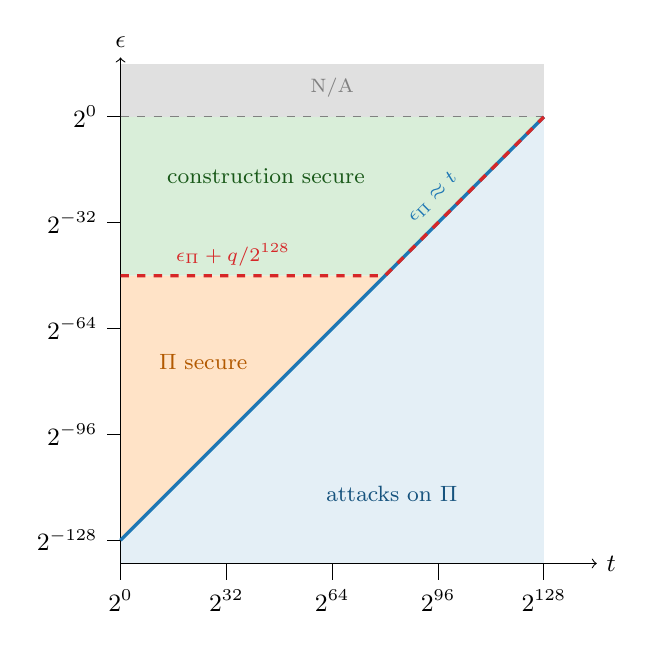
\begin{tikzpicture}[bitsec]
    \def\n{128}
    \fill[black!12]  (0,0) -- (0,16) -- (\n,16) -- (\n,0) -- cycle;
    \fill[cblue!12]  (0,-\n) -- (\n,0) -- (\n,-135) -- (0,-135) -- cycle;
    \fill[orange!22] (0,-\n) -- (0,-48) -- (80,-48) -- cycle;                 % gap
    \fill[cgreen!18] (0,0) -- (0,-48) -- (80,-48) -- (\n,0) -- cycle;          % construction secure
    \draw[->] (0,-135) -- (0,18) node[above] {$\epsilon$};
    \draw[->] (0,-135) -- ({\n+16},-135) node[right] {$t$};
    \foreach \x in {0,32,64,96,128} \draw (\x,-135)--(\x,-140) node[below] {$2^{\x}$};
    \foreach \y in {0,-32,-64,-96,-128} \draw (0,\y)--(-4,\y) node[left] {$2^{\y}$};
    \draw[gray,dashed] (0,0) -- (\n,0);
    \node[gray,font=\scriptsize] at ({0.5*\n},9) {N/A};
    \draw[cblue,very thick] (0,-\n) -- (\n,0);
    \draw[cred,very thick,dashed] (0,-48) -- (80,-48) -- (\n,0);
    \node[cblue,rotate=45,anchor=south,font=\scriptsize] at (98,-28) {$\epsilon_\Pi \approx t$};
    \node[cred,anchor=south,font=\scriptsize] at (34,-48) {$\epsilon_\Pi + q/2^{128}$};
    \node[cgreen!55!black,align=center,font=\footnotesize] at (44,-18) {construction secure};
    \node[orange!70!black,align=center,font=\footnotesize] at (25,-74) {$\Pi$ secure};
    \node[cblue!70!black,align=center,font=\footnotesize] at (82,-114) {attacks on $\Pi$};
  \end{tikzpicture}
}

%======================================================================
% PANEL 2 :  log t  vs  log eps   --  GROVER / collision
%======================================================================

%======================================================================
% PANEL 3 :  t  vs  kappa   (bit-security view)  --  SEARCH / linear
%======================================================================
\newcommand{\panelKap}{%
  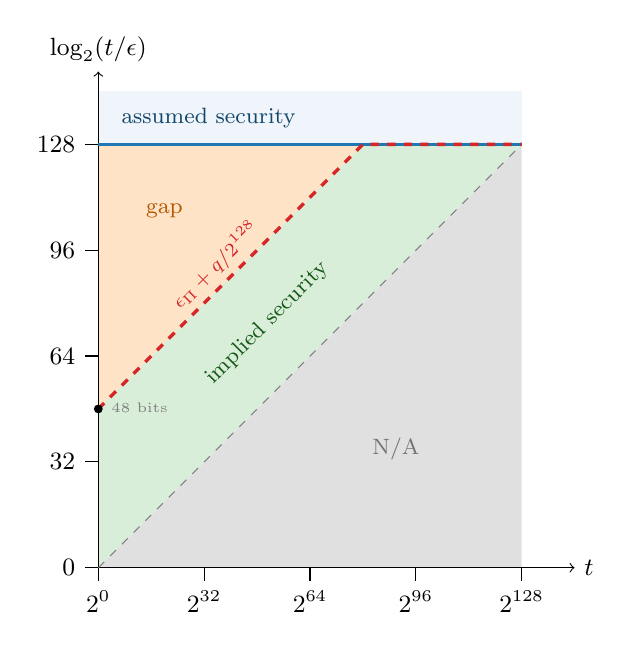
\begin{tikzpicture}[bitsec]
    \def\n{128}
    \fill[cblue!7]   (0,\n) -- (0,{\n+16}) -- (\n,{\n+16}) -- (\n,\n) -- cycle;
    \fill[black!12]  (0,0) -- (\n,\n) -- (\n,0) -- cycle;
    \fill[cgreen!18] (0,0) -- (0,48) -- (80,\n) -- (\n,\n) -- cycle;           % implied (parallel band)
    \fill[orange!22] (0,48) -- (0,\n) -- (80,\n) -- cycle;                     % gap
    \draw[->] (0,0) -- (0,{\n+22}) node[above] {$\log_2(t/\epsilon)$};
    \draw[->] (0,0) -- ({\n+16},0) node[right] {$t$};
    \foreach \x in {0,32,64,96,128} \draw (\x,0)--(\x,-4) node[below] {$2^{\x}$};
    \foreach \y in {0,32,64,96,128} \draw (0,\y)--(-4,\y) node[left] {$\y$};
    \draw[gray,dashed] (0,0) -- (\n,\n);
    \draw[cblue,very thick] (0,\n) -- (\n,\n);
    \draw[cred,very thick,dashed] (0,48) -- (80,\n) -- (\n,\n);
    \fill (0,48) circle (1.6pt);
    \node[anchor=south west,font=\tiny,gray] at (1,44) {$48$ bits};
    \node[cblue!60!black,anchor=west,font=\footnotesize] at (4,{\n+8}) {assumed security};
    \node[cred,rotate=45,anchor=south,font=\scriptsize] at (40,87) {$\epsilon_\Pi+q/2^{128}$};
    \node[orange!70!black,font=\footnotesize] at (20,108) {gap};
    \node[cgreen!55!black,rotate=45,font=\footnotesize] at (51,74) {implied security};
    \node[black!55,align=center,font=\footnotesize] at (90,36) {N/A};
  \end{tikzpicture}
}

%======================================================================
% PANEL 4 :  t  vs  kappa   --  GROVER / collision
%======================================================================

\begin{tabular}{@{}c@{\hspace{3em}}c@{}}
  %\panelcap{\panelEpsSearch}{
  \panelcap{\panelEps}{
    %(a) Possible attacks if best attack against the
    %primitive scales linearly with time (brute-force)
    (a) Ruled-out attacks if the best attack on the primitive scales
    \emph{linearly} (brute-force)
  %}
  % & \panelcap{\panelEpsGrover}{
  %  (b) vs.\ \emph{quadratically} (birthday/Grover)
  }\\[30pt]
  %\panelcap{\panelKapSearch}{
  \panelcap{\panelKap}{
    %(c) Bit security if best primitive attack $=$ brute-force
    (c) Bit security if the best attack on the primitive scales
    \emph{linearly} (brute-force)
  }\\
  % & \panelcap{\panelKapGrover}{
  %  (d) vs.\ \emph{quadratically} (birthday/Grover)
  %}\\
\end{tabular}

